\normalfalse \difficiletrue \tdifficilefalse
\correctionfalse
%\UPSTIidClasse{11} % 11 sup, 12 spé
%\newcommand{\UPSTIidClasse}{12}

\exer{Pompe ENSIETA  $\star\star$ \label{CIN:01:B2:12:1020}}
\setcounter{question}{0}\marginnote{\xpComp{CIN}{01}}%\UPSTIcompetence{B2-12}
\index{Compétence B2-12}\index{Compétence CIN-01}
\index{Schéma cinématique}
\index{Pompe ENSIETA}

\ifcorrection
\else
\marginnote{\textbf{Pas de corrigé pour cet exercice.}}
\fi



\ifprof
\else
Le plan joint format A4 représente l’ensemble monté d’une pompe hydraulique manuelle.

La pompe est fixée sur un support vertical au moyen de 3 trous filetés (1). Une série de trois trous filetés est usinée sur chaque coté du corps (2), permettant ainsi de fixer indifféremment la pompe sur l’une ou l’autre de ses faces.

L’admission de l’huile est effectuée par l’orifice (3), le refoulement par l’orifice (4).

Le pompage s’effectue en actionnant un levier placé dans l’alésage cannelé du maneton (5). Le mouvement alternatif est, par l’intermédiaire de la biellette articulée, transmis au piston coulissant (6).

Lors du mouvement de droite à gauche du piston coulissant, un volume d’huile est aspiré à travers (3) et vient s’emmagasiner dans l’alésage à droite de la tête du piston, simultanément l’huile qui se trouve à gauche de la tête du piston est refoulée par l’orifice (4).

Lors du mouvement de gauche à droite du piston coulissant s’effectue le transfert, à travers de la tête du piston, de l’huile emmagasinée à sa droite (celle-ci passant côté tige). Simultanément une partie de l’huile transférée est refoulée dans (4).

Un clapet anti-retour est constitué d’une bille et d’un ressort. Sur la pompe étudiée ils sont au nombre de trois. 
Le passage du fluide dans un sens, par action sur la bille provoque l’écrasement du ressort et libère le passage. 
Dans le sens contraire l’action du fluide se conjugue avec celle du ressort et interdit le passage. 
\fi

\question{Le diamètre nominal de la bille contenue dans le clapet anti-retour situé sur l’orifice (4) est identique à celui de l’alésage qui la guide. Est-ce fonctionnellement correct ? Justifier votre réponse. L’observation de la pièce (7) du clapet situé sur l’orifice (3) peut vous aider pour la réponse.}

\question{L’alésage du corps contenant l’extrémité du raccord orifice (4) et l’alésage sur lequel le piston (6) coulisse doivent-ils être réalisés avec le même type d’état de surface ? Justifier votre réponse.}

\question{Entre la tige du piston et l’alésage du corps, quel ajustement choisir ? Préciser s’il s’agit d’un ajustement avec jeu, avec serrage ou ajusté.}

\question{D’après la représentation du dessin d’ensemble, un des composants de la pompe ne peut pas être monté. Quel est-il (donner son numéro) ? Pourquoi ? Que faudrait-il faire pour le rendre montable ?}

\question{Dans le mouvement de droite à gauche du piston, le volume aspiré dans (3) à droite de la tête de piston est-il le même que celui refoulé à gauche de la tête de piston dans (4) ? Justifier votre réponse.}


\ifprof
\else
On donne les dimensions suivantes :
\begin{itemize}
\item tête de piston = \SI{29}{mm};
\item tige de piston = \SI{18}{mm};
\item course du piston = \SI{31}{mm}.
\end{itemize}
\fi

\question{Quel est le volume d’huile  envoyé à la sortie (4) :}
\textit{
\begin{itemize}
\item lors de la course droite -- gauche du piston ?
\item lors de la course gauche -- droite du piston ?
\end{itemize}}


\ifprof
\else

\subsection*{Schéma cinématique}
On considère la pompe sans aucun clapet. Seule la transformation de mouvement permettant le déplacement du piston nous intéresse.

\fi

\question{Faire le schéma cinématique de la pompe.}


\ifprof
\else
\begin{marginfigure}
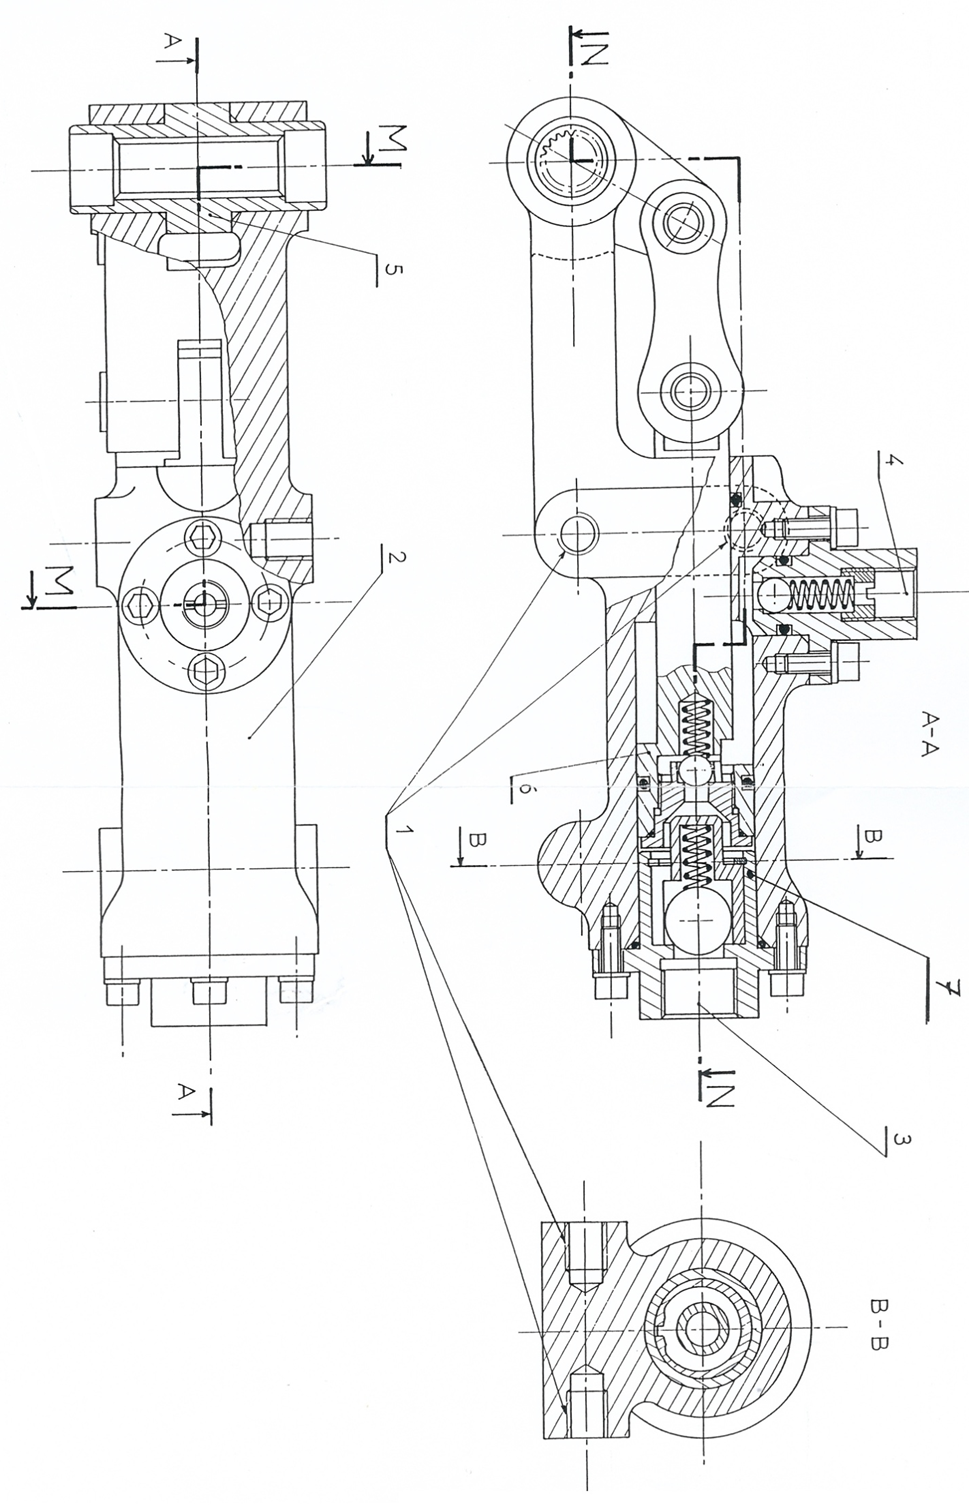
\includegraphics[width=.9\linewidth]{1020_02}
\end{marginfigure}
\fi


\ifprof
\else

\footnotesize
%\begin{marginfigure}
%\begin{tabular}{|p{.9\linewidth}|}
%\hline
%Indications (à vérifier...) :
%\begin{enumerate}
%\item $\vectv{B}{2}{0} = L\varphip(t)\vj{2} +\thetap(t)\left(L\vj{1}-R\vi{0}\right) $.
%\item  $\torseurcin{V}{2}{0} = \torseurl{\vecto{2}{0}=\left( \varphip(t)+\thetap(t) \right) \vk{0} }{ L\varphip(t)\vj{2} +\thetap(t)\left(L\vj{1}-R\vi{0}\right)}{B}$.
%\item $\vectg{B}{2}{0} =  L\varphipp(t)\vj{2}-L\varphip(t)\left(\varphip(t)+\thetap(t) \right)\vi{2}  + \thetapp(t)\left(L\vj{1}-R\vi{0}\right) - L\thetap^2(t)\vi{1}$.
%\end{enumerate} \\ \hline
%\end{tabular}
%\end{marginfigure}
\normalsize



\marginnote{Corrigé  voir \ref{CIN:01:B2:12:1020}.}

\fi